\chapter{Revisión de la literatura}
La selección de características es un problema cuya popularidad ha ido en aumento con el paso de los años. No es algo casual, pues la cantidad de datos recogidos para tareas de aprendizaje automático y áreas derivadas, como el aprendizaje profundo, ha ido en aumento de manera casi exponencial.

\begin{figure}[H]
    \begin{center}
        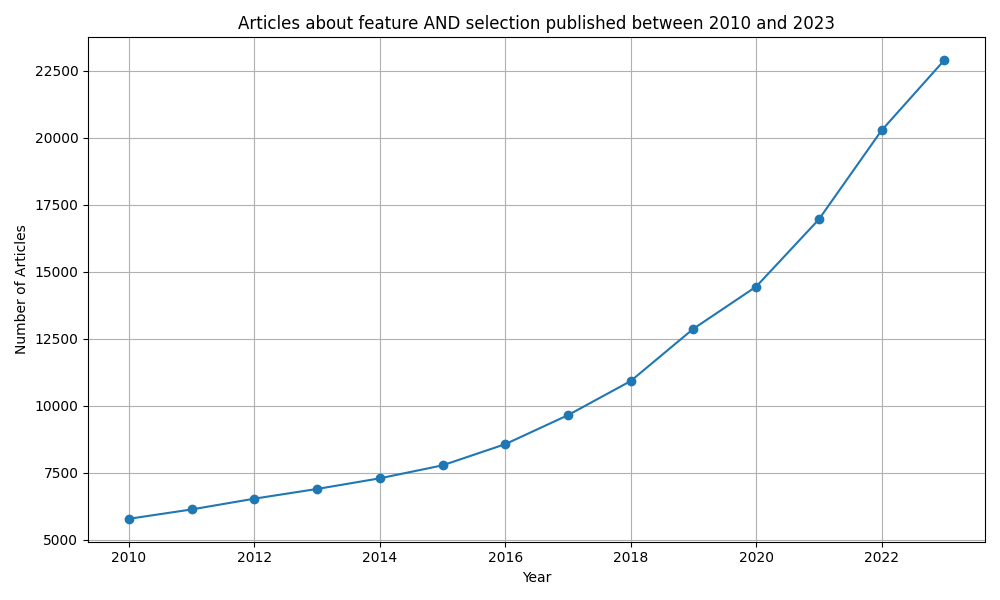
\includegraphics[width=1\textwidth]{imagenes/scopus_chart.png}
    \end{center}
    \caption[Popularidad de feature selection sobre los años]{En esta figura se muestra el número de artículos publicados relacionados con la selección de características. Se ha usado el buscador Scopus para estos resultados.}
    \label{fig:pop_fs}
\end{figure}

También se puede observar una tendencia  prácticamente igual en la popularidad sobre los años del problema de selección de características, pero abordado con técnicas metaheurísticas.

\begin{figure}[H]
    \begin{center}
        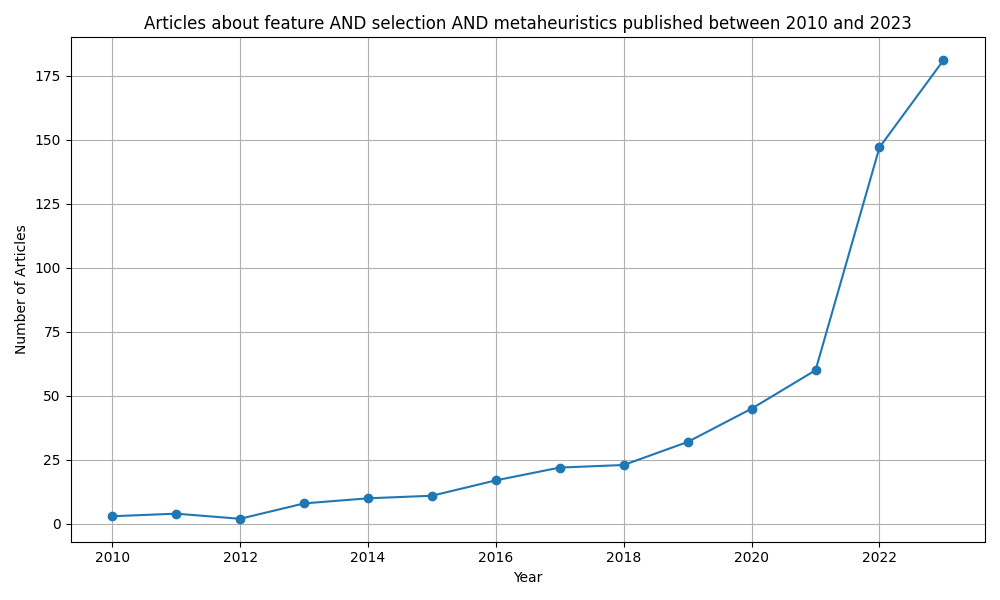
\includegraphics[width=1\textwidth]{imagenes/scopus_chart2.png}
    \end{center}
    \caption[Popularidad de feature selection + metaheuristics sobre los años]{De igual forma que en la figura \ref{fig:pop_fs} las mateheuristicas han ido muy ligadas a la resolución de este problema. Se ha usado el buscador Scopus para estos resultados.}
\end{figure}
Y es que las metaheurísticas son algoritmos muy convenientes en la resolución de este tipo de problemas. Algoritmos analíticos no son válidos cuando el conjunto de datos tiene un número de características muy elevado debido a una cantidad de combinaciones simplemente inabordable en términos computacionales. Debido a ello, se suelen utilizar algoritmos más rápidos cuya solución no es óptima en términos globales, pero si suficientemente buena.\\[6pt]
Muchos algoritmos metaheurísticos han sido propuestos a lo largo de los años. Se han escogido los más destacables en cuanto a resultados y más mencionados entre todos ellos, dando una selección de algoritmos metaheurísticos modernos de, en principio, muy alta calidad. No solo son seleccionados algoritmos modernos, sino que también se han escogido una serie de algoritmos más ``clásicos'', pero cuya aplicación es más extendida y con resultados que, de forma empírica, han demostrado ser más que buenos a lo largo de décadas de uso.

\begin{table}[H]
    \parbox{.45\linewidth}{
        \centering
        \begin{tabular}{l}
            \hline
            Algoritmos \\ \hline
            GWO        \\
            FA         \\
            GOA        \\
            WOA        \\
            DA         \\
            CS         \\
            BA         \\
            \hline
        \end{tabular}
        \caption{Algoritmos modernos}
    }
    \hfill
    \parbox{.45\linewidth}{
        \centering
        \begin{tabular}{l}
            \hline
            Algoritmos \\ \hline
            PSO        \\
            GA         \\
            ACO        \\
            DE         \\
            ABCO       \\
            \hline
        \end{tabular}
        \caption{Algoritmos clásicos}
    }
\end{table}

Los algoritmos usados en este proyecto pertenecen todos a la sub-categoría conocida como algoritmos poblacionales, esto es, algoritmos que parten de un conjunto de soluciones inicializadas de forma aleatoria y representadas en forma de vectores llamadas población. Este tipo de algoritmos ``evolucionan'' durante un número de generaciones hasta alcanzar un máximo número de generación o alcanzar un miembro de la población cuya solución sea lo suficientemente buena~\cite{simon2013evolutionary}.

\section{Introducción a los primeros algoritmos poblacionales}

Uno de los primeros algoritmos basados en poblaciones y evolutivos es el algoritmo genético. Los algoritmos genéticos o \textit{GAs} ganaron popularidad en los años $70$, particularmente en $1975$ con el libro de John Holland~\cite{Holland:1975}. Este tipo de metaheurísticas son diseñadas basándose en la selección natural. Un conjunto de fenotipos (soluciones) son evolucionadas durante generaciones para emular el cruce entre especies (cruce de soluciones mediante un intercambio común de cromosomas) dando lugar a nuevos individuos con características de ambos padres. Poco a poco este tipo de algoritmos fueron desarrollando nuevas características y aunque en un principio fueron diseñados para resolver problemas discretos, también tienen versiones que optimizan problemas continuos~\cite{eiben2015}.\\[6pt]
Uno de los primeros algoritmos metaheurísticos basados en poblaciones es el \textit{sistema de hormigas} de Dorigo, que fue presentado en $1991$~\cite{as}. Esta metaheurística fue aplicada a la resolución del problema del vendedor ambulante con resultados muy prometedores, pues resolvía el problema de forma muy eficiente con una solución sub-óptima, pero suficientemente buena. A partir de este punto, surgieron numerosas mejoras y versiones de los algoritmos basados en colonias de hormigas.\\[6pt]
Más tarde se presentó el conocido algoritmo de \textit{optimización por enjambre de partículas}, nombrado como \textit{PSO} por sus siglas en inglés y presentado por Kennedy y Eberhart en $1995$~\cite{kennedy_particle_1995}. El algoritmo \textit{PSO} surgió a partir de la observación del comportamiento social de las aves y peces. La idea principal del \textit{PSO} es que cada solución candidata (o ``partícula'') en el espacio de búsqueda se mueve a través del espacio en función de su propia mejor posición conocida y la mejor posición conocida de cualquier partícula en el enjambre, en lugar de depender de operadores de búsqueda convencionales. El algoritmo comenzaba con un conjunto de soluciones candidatas aleatorias, denominadas partículas, que procedian a moverse a través del espacio de búsqueda para encontrar la solución óptima. Cada partícula tenía una posición y una velocidad asociadas.\\[6pt] 
En $1999$ se presentó el conocido \textit{ACO} u \textit{optimización de colonia de hormigas}~\cite{dorigo_ant_1999}. Este algoritmo refinada la fórmula anteriormente usada en \textit{AS} usando un grafo como representación del conjunto de soluciones, la actualización y rastro de feromona como heurística principal para escoger el camino en el grafo y una codificación discreta de las características.\\[6pt]
La \textit{evolución diferencial} fue un algoritmo de optimización propuesto por primera vez por Rainer Storn y Kenneth Price en el año $1997$~\cite{storn_differential_1997}. Surgió como una alternativa a los algoritmos genéticos existentes en ese momento, ya que se inspiraba en su diseño, pero siendo inicialmente diseñado para resolver problemas continuos, a diferencia de los \textit{GAs}.\\[6pt]
La idea detrás de la evolución diferencial se basaba en la exploración de un espacio de búsqueda mediante la manipulación de vectores de parámetros. A diferencia de los \textit{GAs}, que utilizaban operadores genéticos como la cruza y la mutación, la \textit{DE} se centraba principalmente en la mutación basada en la diferencia entre vectores de la población. Inicialmente, el algoritmo atrajo la atención debido a su simplicidad y eficiencia en la optimización de funciones complejas en espacios de búsqueda continuos.\\[6pt]
El algoritmo de optimización basado en colonias de abejas es considerado otro gran clásico de las metaheurísticas poblacionales bio-inspiradas, pese a ello, es el más nuevo de los ya mencionados. El algoritmo de colonias de abejas artificiales o \textit{ABCO} fue propuesto por primera vez por Dervis Karaboga en $2005$~\cite{karaboga_idea_nodate}. Surgió como una técnica inspirada en el comportamiento de las colonias de abejas para resolver problemas de optimización y se basaba en imitar el comportamiento de las abejas en la búsqueda de alimentos. En la naturaleza, las abejas utilizan la danza de reclutamiento para comunicar la ubicación de las fuentes de alimento a otras abejas en la colmena. Karaboga adaptó este proceso en un algoritmo de optimización que utiliza abejas artificiales para explorar y explotar un espacio de búsqueda.

\section{Propuestas metaheurísticas modernas}
\begin{figure}[H]
    \centering
    \begin{subfigure}[b]{0.45\textwidth}
      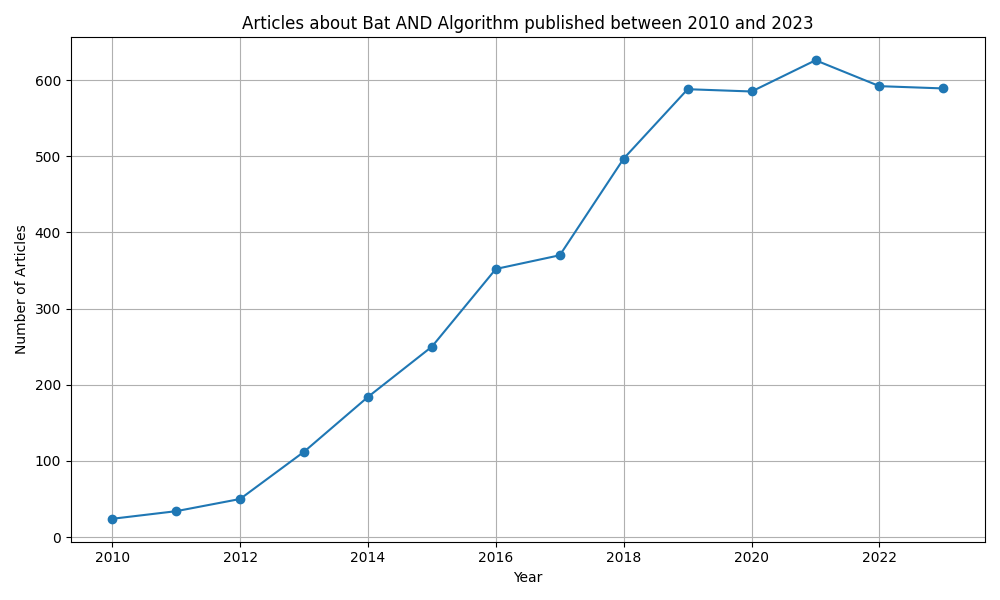
\includegraphics[width=\textwidth]{imagenes/scopus_chart_Bat_Algorithm.png}
      \caption{BA}
      \label{fig:bat_algorithm}
    \end{subfigure}
    \begin{subfigure}[b]{0.45\textwidth}
      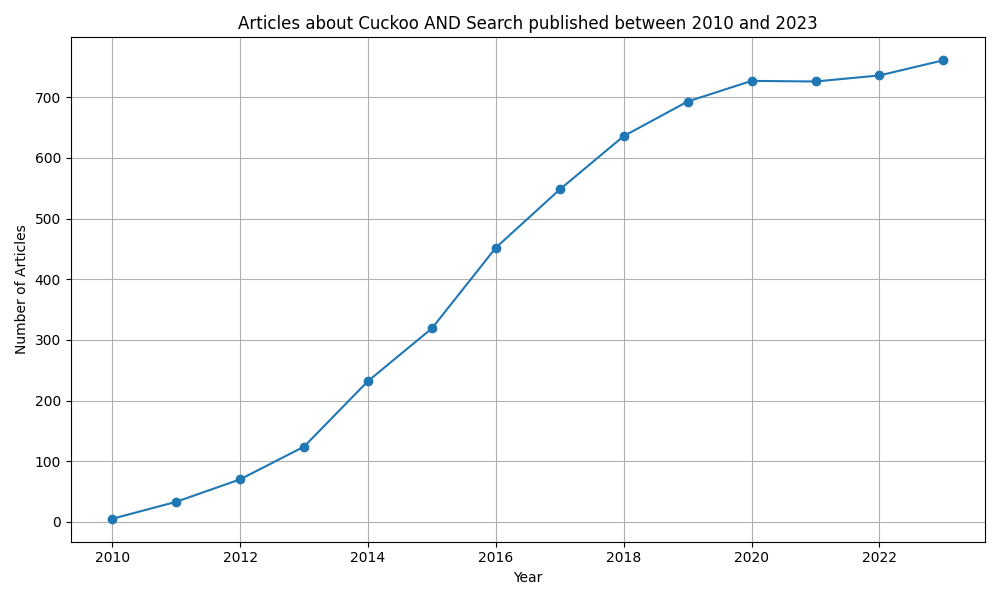
\includegraphics[width=\textwidth]{imagenes/scopus_chart_Cuckoo_Search.png}
      \caption{CS}
      \label{fig:cuckoo_search}
    \end{subfigure}
    \begin{subfigure}[b]{0.45\textwidth}
      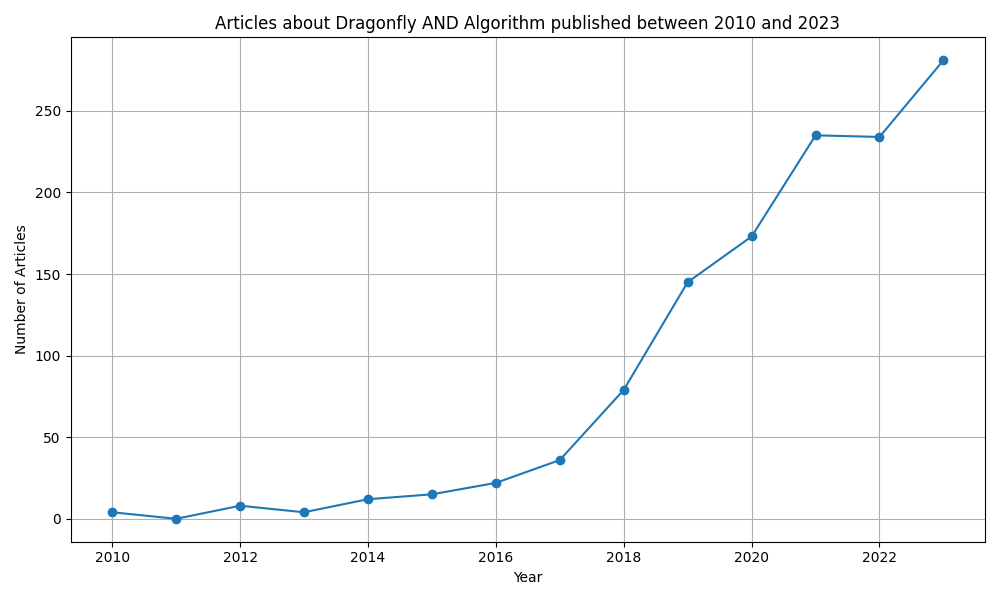
\includegraphics[width=\textwidth]{imagenes/scopus_chart_Dragonfly_Algorithm.png}
      \caption{DA}
      \label{fig:dragonfly_algorithm}
    \end{subfigure}
    \vspace{0.5cm} % Espacio vertical entre filas de imágenes
    \begin{subfigure}[b]{0.45\textwidth}
      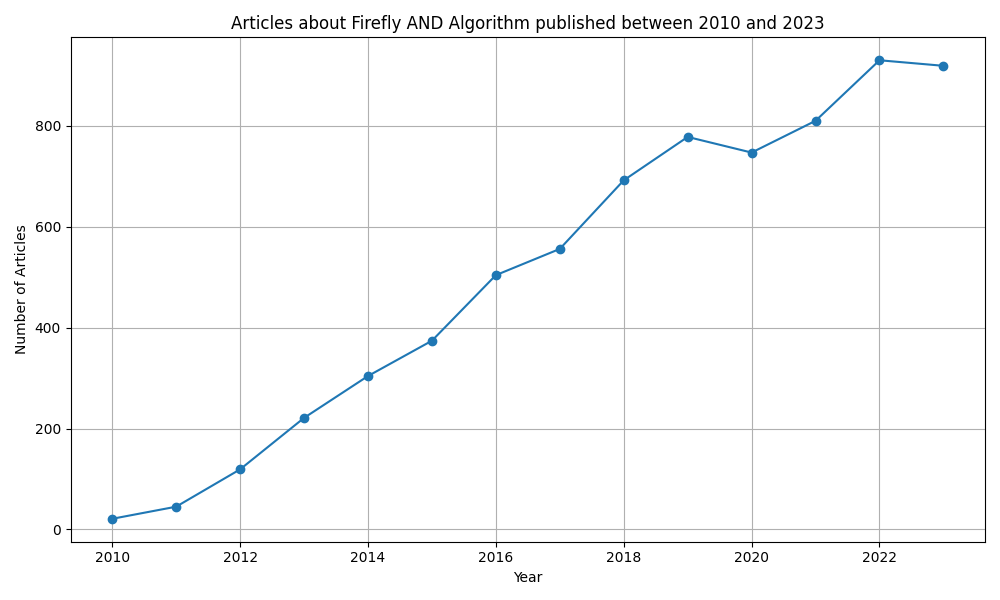
\includegraphics[width=\textwidth]{imagenes/scopus_chart_Firefly_Algorithm.png}
      \caption{FA}
      \label{fig:firefly_algorithm}
    \end{subfigure}
    \begin{subfigure}[b]{0.45\textwidth}
      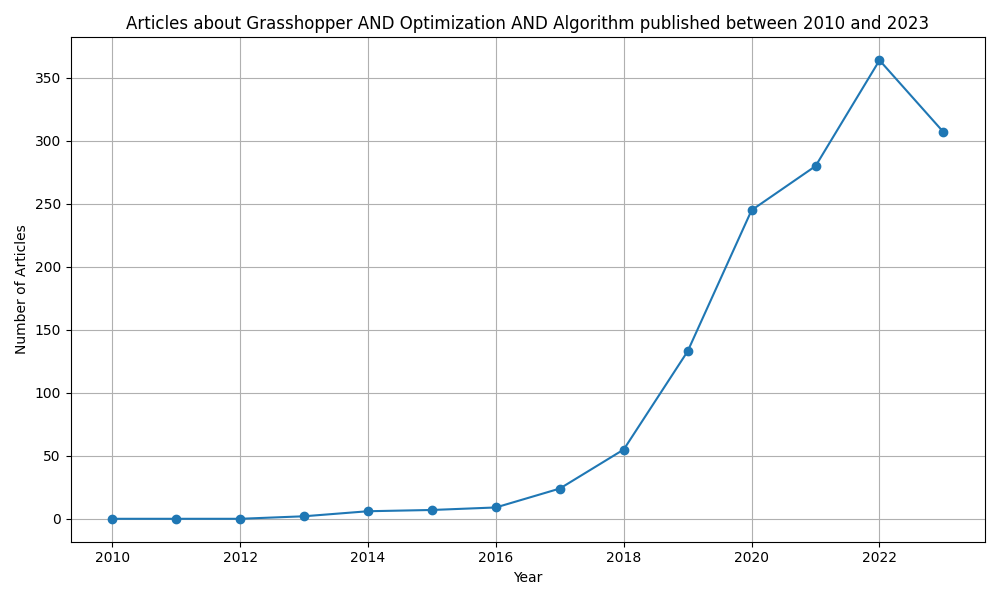
\includegraphics[width=\textwidth]{imagenes/scopus_chart_Grasshopper_Optimization_Algorithm.png}
      \caption{GOA}
      \label{fig:grasshopper_algorithm}
    \end{subfigure}
    \begin{subfigure}[b]{0.45\textwidth}
      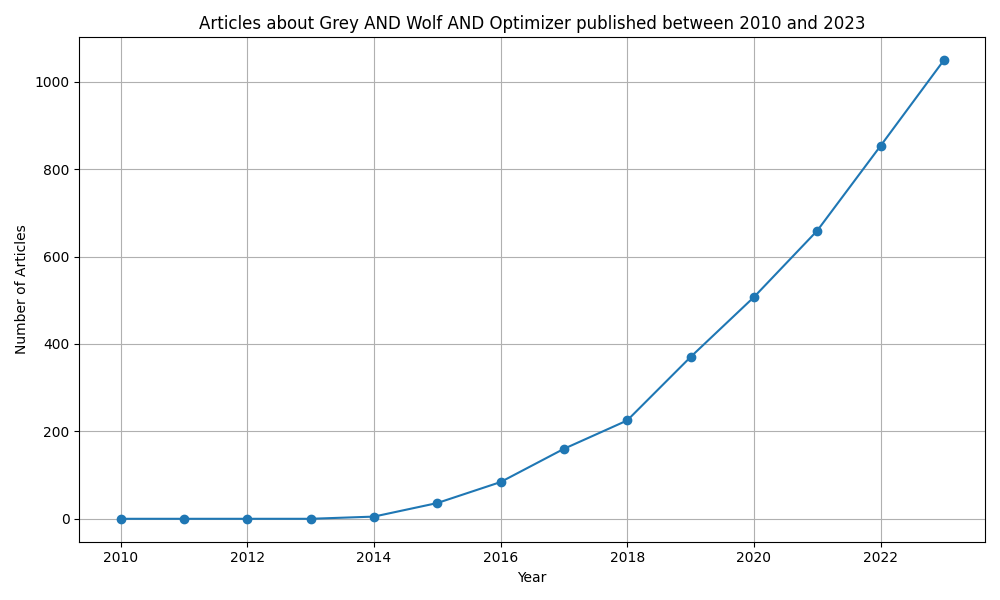
\includegraphics[width=\textwidth]{imagenes/scopus_chart_Grey_Wolf_Optimizer.png}
      \caption{GWO}
      \label{fig:grey_wolf_optimizer}
    \end{subfigure}
    \vspace{0.5cm} % Espacio vertical entre filas de imágenes
    \begin{subfigure}[b]{0.45\textwidth}
      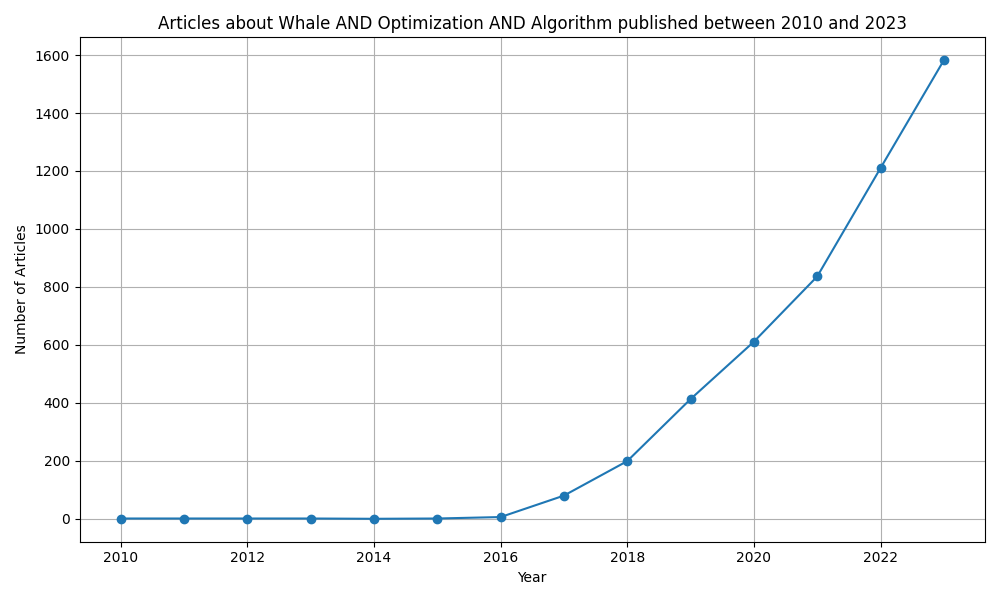
\includegraphics[width=\textwidth]{imagenes/scopus_chart_Whale_Optimization_Algorithm.png}
      \caption{WOA}
      \label{fig:whale_optimization_algorithm}
    \end{subfigure}
    \caption[Popularidad metaheurísticas modernas]{Número de búsquedas en Scopus de los diferentes algoritmos metaheurísticos seleccionados. Se puede ver una clara tendencia alcista en la popularidad de estos pese a su relativa novedad en el campo de la optimización.}
    \label{fig:conjunto_imagenes}
\end{figure}
